% moxi.tex:

\chapter{MOBILE-PHONE-BASED OXIMETER (MOXI)} % all caps please
\label{chap:moxi}


\section{Introduction} %significan
\label{chap:moxi:introduction}
Every year, nearly 3 million newborns die within the first 4 weeks of life in \ac{LMIC}s~\cite{Worldhealthorganization2006}. Respiratory complications, such as birth asphyxia, and congenital heart defects, such as Tetralogy of Fallot (which results in Blue Baby Syndrome – a condition caused by low tissue oxygenation), are among the major causes of death at birth for neonates. In addition, over 17\% of the post-neonatal child deaths are caused by childhood pneumonia and other acute respiratory infections, accounting for 4 million deaths per year for children under age 5~\cite{Alexander2018}. These conditions often lead to low arterial and tissue oxygenation~\cite{Weber2003}. Many of these complications are easily screened, diagnosed, and continuously monitored in most facilities in developed countries using a pulse oximeter, a device to measure arterial blood oxygen levels (SpO2) using low-power light based on NIRS. 

Finger-clip-based pulse oximeters, however, are difficult to use on small fingers. Newborn specific pulse oximeter probes, often sold as disposable parts, can cost up to \$100 USD, and require a more expensive oximeter system to read and display results~\cite{Ouro-BangnaMaman2005,Heywood1989}. These designs thus have extremely limited presence in first-level clinics in LMICs. In recent years, portable NIR devices have been reported, but they generally have high costs dues to sensitive charge-coupled device (CCD) cameras and stand-alone image acquisition software~\cite{Jung2013}, or still require the use of a finger-clip~\cite{Karlen2011,Hudson2012}. Many factors, primarily high acquisition and maintenance costs (Table~\ref{tab:lmicbarriers}), have hindered the adoption of portable diagnostics tools~\cite{Malkin2007}. 

\begin{table}[]
\centering
\caption{Barriers to adoption of new medical devices in LMICs}
\label{tab:lmicbarriers}
\begin{tabular}{@{}cl@{}}
\toprule
Rank & Barrier to Adoption \\ \midrule
1    & Acquisition Costs   \\
2    & Spare Parts         \\
3    & Consumables         \\
4    & Reliable Power      \\
5    & Infrastructure      \\
6    & Training            \\ \bottomrule
\end{tabular}
\end{table}

A silver lining comes from the Pew Global Research Center, which reported that smartphone ownership in \ac{LMIC}s rose from 21\% to 45\% between 2013 and 2018, making smartphone networks the fastest growing infrastructure in LMICs~\cite{Poushter2016}. By capitalizing on the ubiquitous presence of smartphones worldwide, we aim to develop phone-camera based and phone-communication facilitated NIRS devices to measure tissue oxygenation, directly addressing the barriers to adoption in Table~\ref{tab:lmicbarriers}. These smartphone-based devices can address the current limitations of conventional pulse oximeters, including newborn-unfriendly clip designs, acquisition and maintenance costs of disposable probes, and the need for frequent disinfection due to direct skin contact. Leveraging smartphone features such as cameras, LEDs, and wireless communication along with their power and computation will pave the way for POC smartphone-based diagnostic tools. 

\begin{figure}
	\begin{center}
	\subfigure[]{\label{fig:moximeter}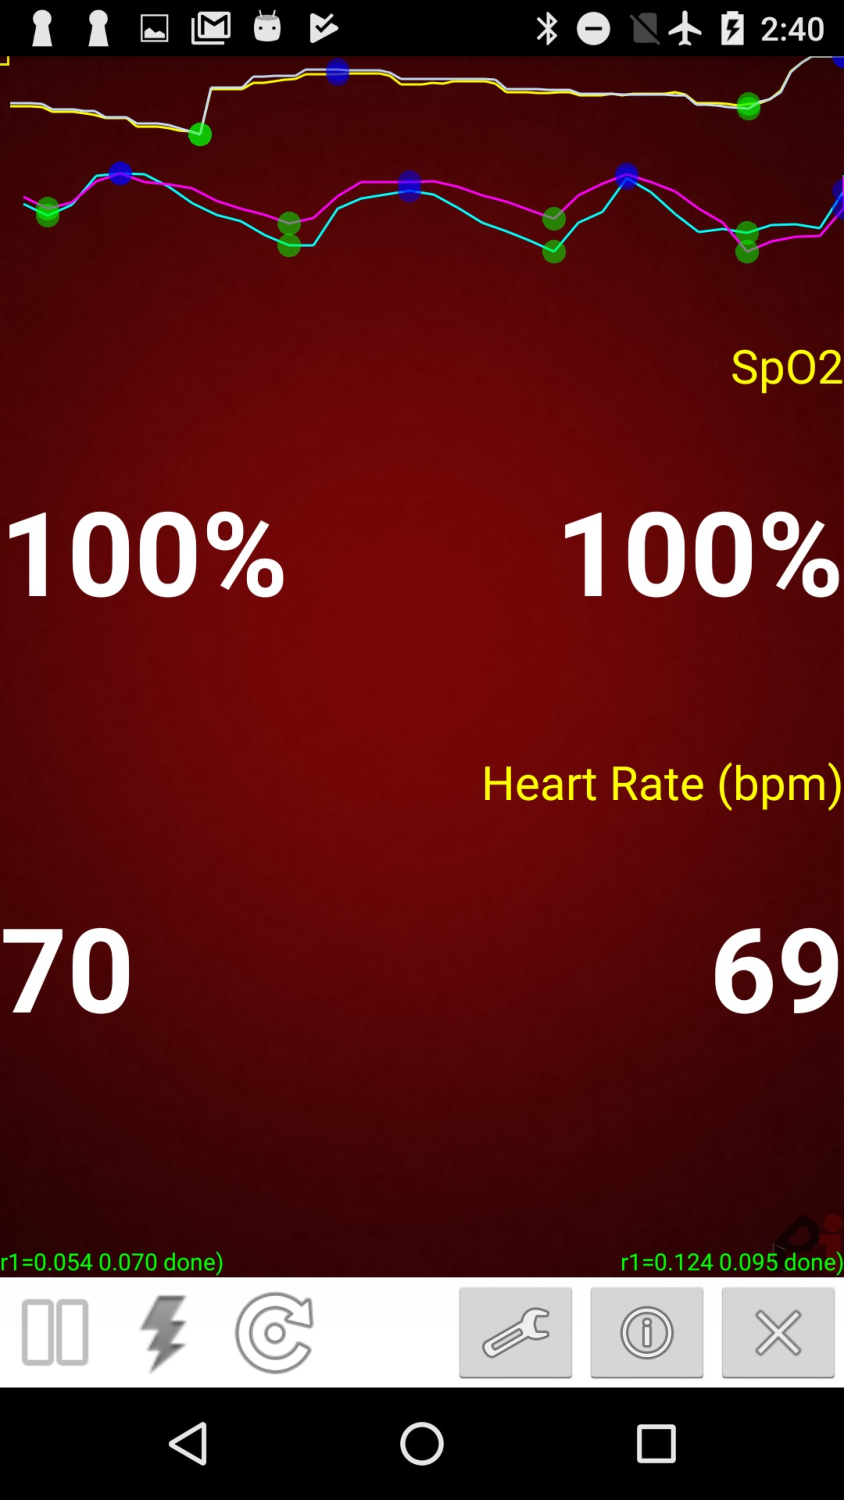
\includegraphics[height=6cm]{fig/moxi/moximeter.pdf}}
	\subfigure[]{\label{fig:D1D3}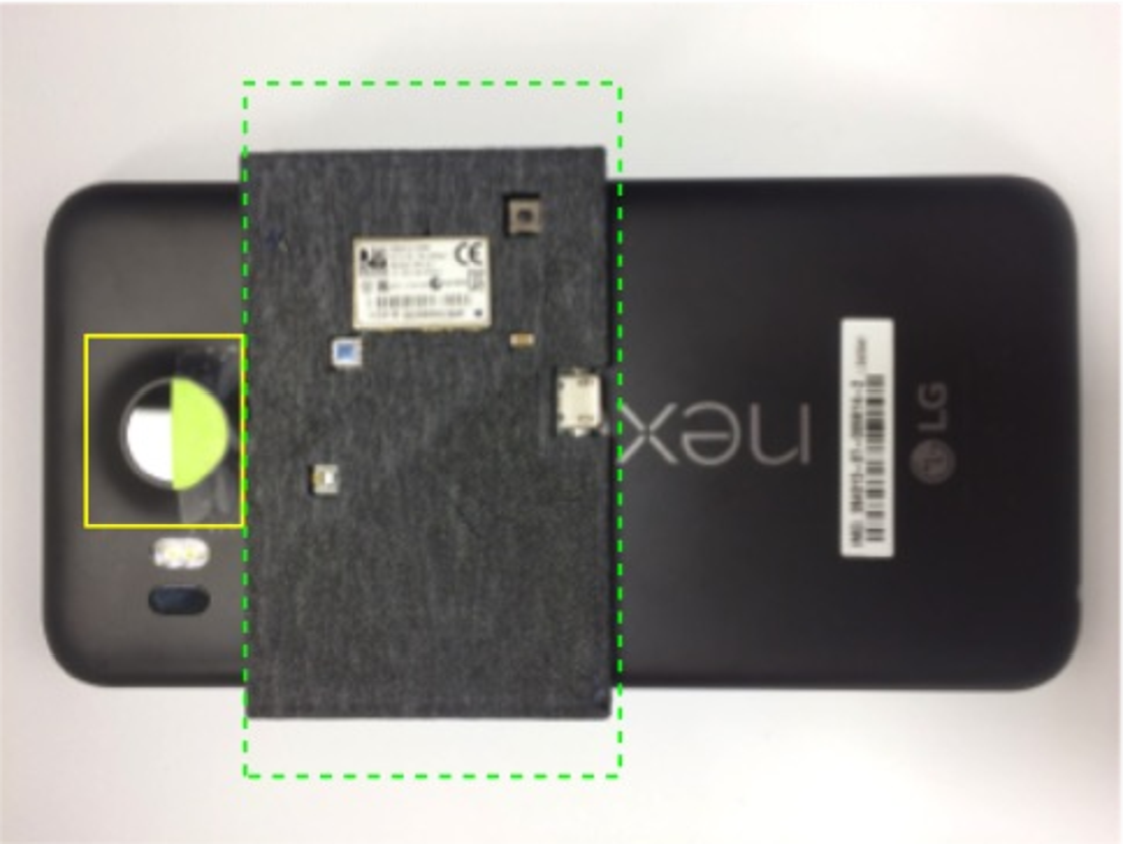
\includegraphics[height=6cm]{fig/moxi/D1D3.pdf}}
	\subfigure[]{\label{fig:D2}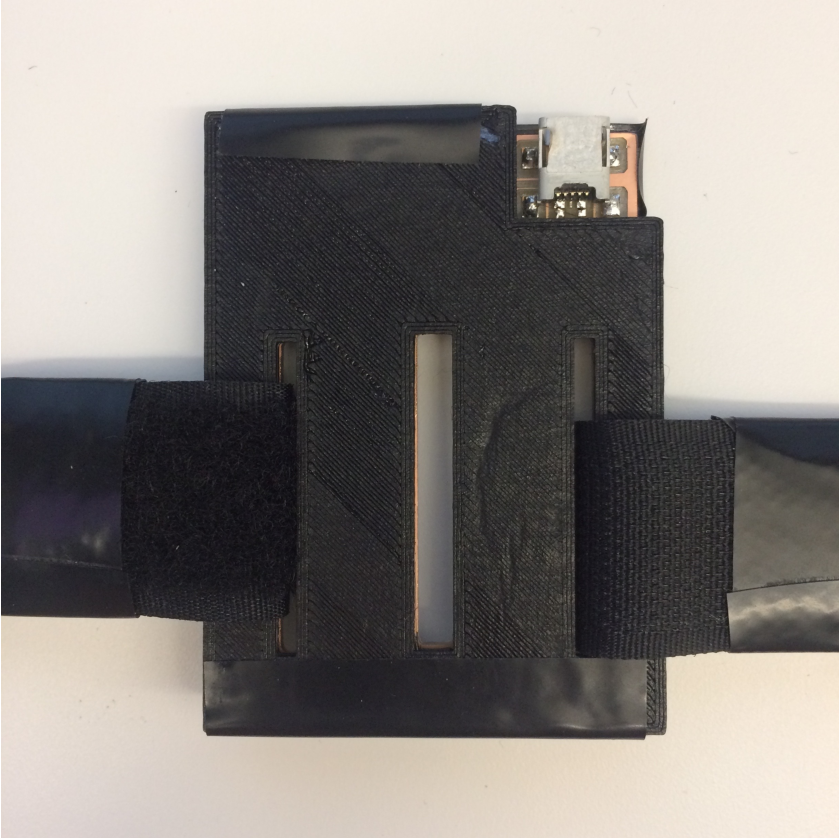
\includegraphics[height=6cm]{fig/moxi/D2.pdf}}
	\end{center}
	\caption{(a) Screenshot of Moximeter mobile application simultaneously capturing D1 and D3 data. (b) D1 (green, dashed) and D3 (yellow, solid) mounted on a smartphone phone. (c) D2 board with cover.} 
	\label{fig:designs}
\end{figure} 

In this chapter, we establish the feasibility and accuracy of three smartphone-based approaches to monitoring oxygenation. In order of decreasing complexity of hardware, the first design (D1) is a Bluetooth wireless oximeter board with a dedicated pulse oximetry chip [Figure~\ref{fig:D1D3}]. The second design (D2) measures tissue oxygen saturation (StO2). It functions by imaging light attenuation in tissue through a slit on a circuit board carrying LEDs [Figure~\ref{fig:D2}]. The third design (D3) is a paper filter covering half of the field of view of a smartphone camera [Figure~\ref{fig:D1D3}]. Both D1 and D3 designs utilize our in-house developed mobile phone application [Figure~\ref{fig:moximeter}] to monitor heart rate (HR) and arterial oxygen saturation (SpO2). The three devices, along with a screenshot of the mobile phone application, are seen in the figure below. Although we include details on D1 and D2 for completeness, when we refer to the \ac{MOXI} system, we are referring to the D3 design. 



%%% Section %%% 
\section{D1: Bluetooth Reflectance Pulse Oximeter}
\subsection{D1: Reflectance Board Hardware}
The D1 design works similarly to a clinical-quality pulse oximeter, except the optodes are placed on the same side of the finger. A photodiode captures the diffuse reflection of the light emitted from two on-board LEDs (640 and 940~nm) in order to estimate SpO2. This reduced form factor, non-finger-clip design makes pulse oximetry measurements more newborn friendly. The D1 board makes use of a low-cost (\$3.5 USD) dedicate pulse oximeter signal-processing chip (AFE4490 Integrated Analog Front-End, Texas Instruments, USA) and a microcontroller (ATMega32u4, Atmel, USA) communicating via the serial-peripheral interface (SPI) communication protocol. The 40x40~mm$^2$ rigid printed circuit board (PCB) can be battery powered or powered by a mobile phone using a male-to-male USB cable. 
    
\subsubsection{Optode settings for Neonates}
In reflectance measurements, the distance between the sources and detector determines the depth of photon propagation. Given the larger fingers of adults compared to neonates in our initial studies (MGH IRB approval is for use on adults with subsequent test on neonates), the current reflectance board has optodes optimized for an adult finger by using a large source-detector (SD) distance of 17~mm. This was empirically chosen based on sweeping the SD distance from 2.54 to 15.24~mm in 2.54~mm increments (0.1 inches to 0.6 inches in 0.1 inch increments based on the breakout board). The highest signal-to-noise ratio (SNR) at this distance was obtained when driving the LEDs at 25~mA. Both 10 mA and 50 mA resulted in smaller amplitudes of the AC component of the signals due to low photon detection and photodiode saturation, respectively. The same trend is seen with the SD distance where being too close or too far leads to weak signals or photodiode saturation. Although set to 17~mm for the pilot rests with adults, when used on neonates, the SD distance should be decreased to account for their smaller finger sizes. 

\subsubsection{Phone Mount}
\begin{figure}
    \begin{center}
    \subfigure[]{\label{fig:D1mount}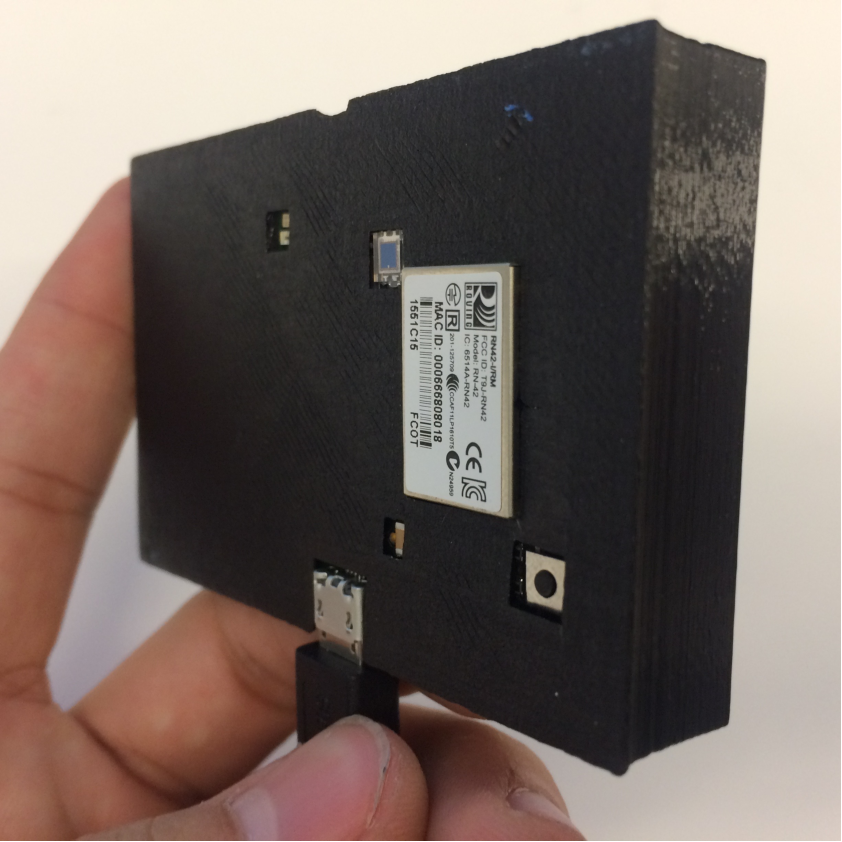
\includegraphics[height=5cm]{fig/moxi/D1mount.pdf}}
    \subfigure[]{\label{fig:D1D3mount}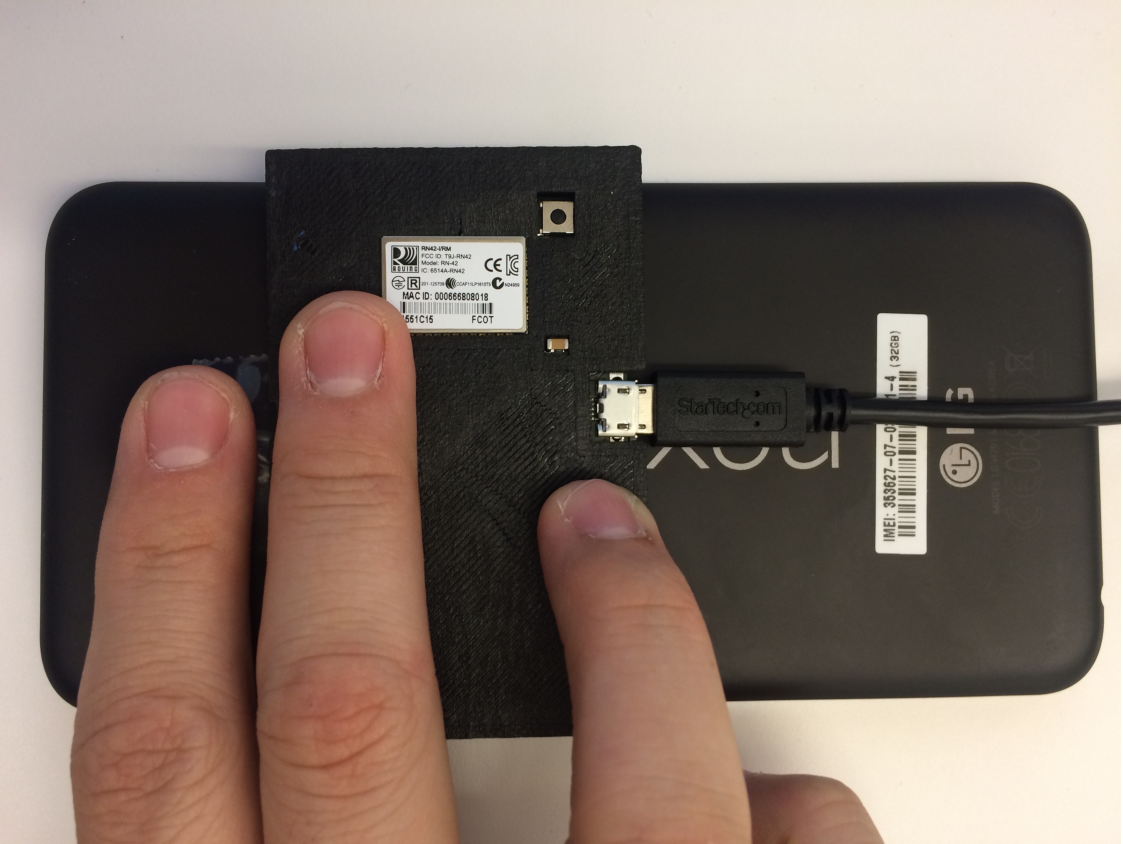
\includegraphics[height=5cm]{fig/moxi/D1D3mount.pdf}}
    \end{center}
    \caption{(a) D1 phone mount. (b) Simultaneous capture of D1 and D3.} 
    \label{fig:D1hardware}
\end{figure} 
The D1 board is placed over a Nexus 5X smartphone using a custom mount [Figure~\ref{fig:D1mount}]. The mount not only holds the D1 board onto the phone, but also prevents users from touching active electronics of the printed circuit board (PCB). The mount is 3-D printed out of Polylactic Acid (PLA). The side panels that grip onto the phone have gaps design to avoid accidentally pressing the volume and power buttons on the sides of the smartphone. The D1 board is press fit onto two small round tabs on the inside, eliminating the need for extra tools. The flat side of the mount is 0.2mm thick to allow maximum surface contact of the optodes onto the finger. Holes on the mount allow access to the reset button of the board, as well as allow the Bluetooth chip to protrude outside for better signal quality. The D1 board is mounted off center to the smartphone to accommodate the longer length of the middle finger compared to the index finger. This allows both fingers to lay comfortably flat during simultaneous capture of D1 and D3 signals [Figure~\ref{fig:D1D3mount}]. The D1 board is powered by a USB male-to-male cable connecting the board to the smartphone’s battery. 

\subsection{D1: Reflectance Board Software}
An Android phone application called Moximeter, written in Java, was developed to process the received signals from the D1 and display the results on the phone. Register values of the AFE4490 were set to 25 mA to each optode and a 500~Hz corner filter was applied post amplification. A long pulse repetition frequency of 250~Hz allows for dynamic averaging of 16 samples per data point by the analog-to-digital converter (ADC) to increase SNR. Bluetooth communication transmits data between the D1 board and the phone. The phone application displays the signals for the red and IR channels at the top of the screen. The signal sample-per-second (in Hz) is dynamically estimated and the PPG waveforms are process in real-time using embedded C-code for maximum efficiency to obtain the oxygen saturation values. The real-time signal processing includes a built-in signal filtering algorithm, peak detection, and algorithm to estimate HR, and an algorithm to compute SpO2 using a transmission pulse oximeter calibration model~\cite{Bailey2008}. The real-time HR and SpO2 values are displayed in the GUI [Figure~\ref{fig:moximeter}]. 
    
\subsubsection{Noise Removal}
Unlike a transmission finger clip where the optodes and finger are coupled, a reflectance-based measurement is more prone to noise and artifacts since the finger being sampled can move independently of the optodes. To reduce this noise, 16 readings of red and IR readings are sampled by the AFE4490 prior to sending an average value to Moximeter. The sampling is done on-board to maintain our 60~Hz sampling rate. Additionally, a 5~ms delay has been added between the SPI transfer calls by the microcontroller to allow the AFE4490 to stabilize. This stabilization prevents loss of data and decreases the likelihood of garbled measurements. As an added precaution, our processing of data workflow now incorporates a mean filter in addition to our band pass filter to remove any unwanted ``chirps'' or spikes in data. 
        
\subsubsection{Independent Source Control}
Photodiodes have a peak wavelength sensitivity and source-pairs have different power outputs from their red and IR LEDs for the same input current. Therefore, the ability to independently adjust each source transmission and receiving channel allows us to obtain comparable signals from the different optodes to increase the sensitivity of our SpO2 calculations.

The receiver channel of the AFE4490 is made up of a differential current-to-voltage trans-impedance amplifier followed by a current digital-to-analog converter (DAC). The amplifier has programmable a feedback resistor ($R_F$) and capacitor ($C_F$) to form a low-pass filter for the input signal current. The output voltage of the amplifier includes the AC component and a component resulting from ambient light leakage. The DAC attempts to amplify only the AC component of the pleth signal. By systematically varying $R_F$, $C_F$, DAC, and the transmitter reference voltage for each optode, we are able to determine the AFE4490 configuration that maximizes the AC components of both red and IR PPG signals, independently. Since the ratio-of-ratios, RR, is based on the amplitude of the AC component of the PPG signals, increasing the AC range with optimized AFE4490 configurations allows for more sensitivity in R calculations and thus more accuracy in SpO2 readings. 
        
\subsection{D1 Results}
\begin{figure}
    \begin{center}
    \subfigure[]{\label{fig:D1resultsa}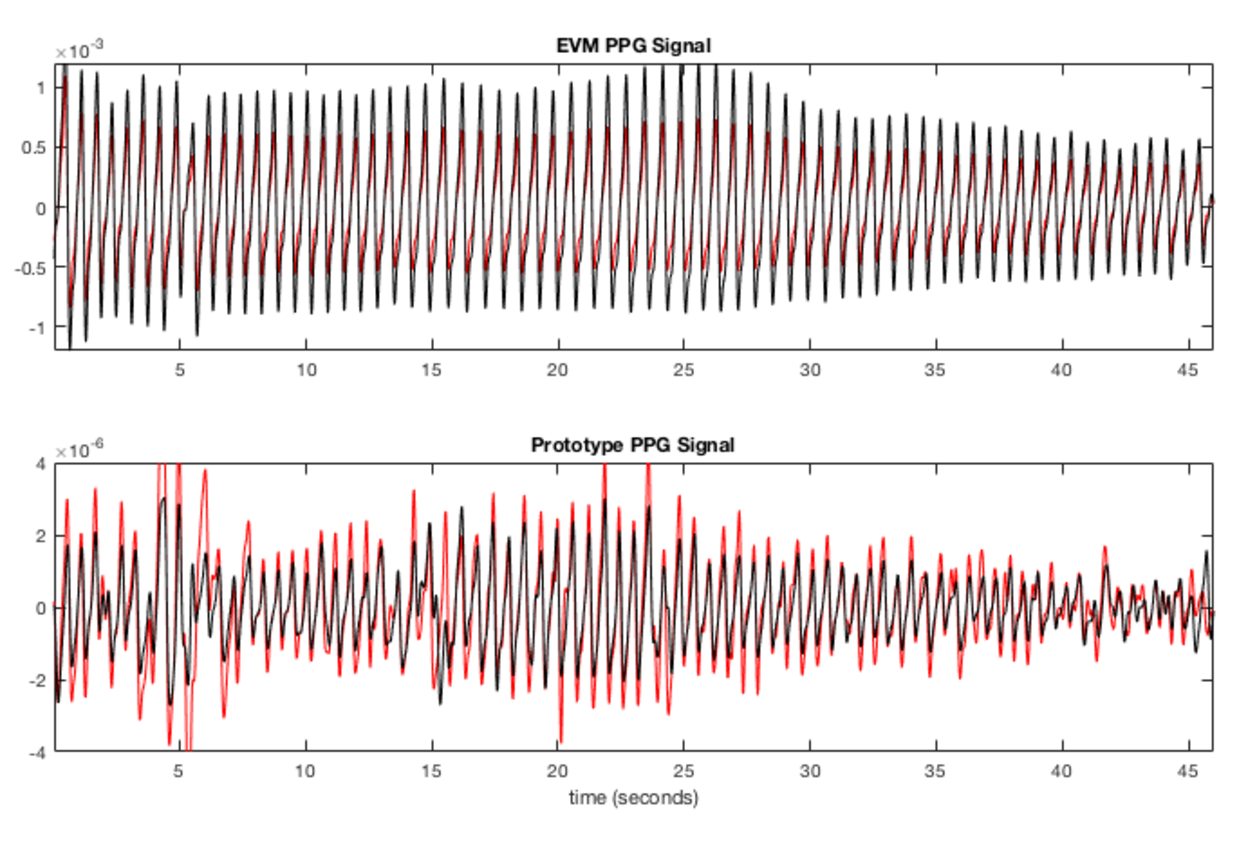
\includegraphics[width=.49\textwidth]{fig/moxi/D1resultsa.pdf}}
    \subfigure[]{\label{fig:D1resultsb}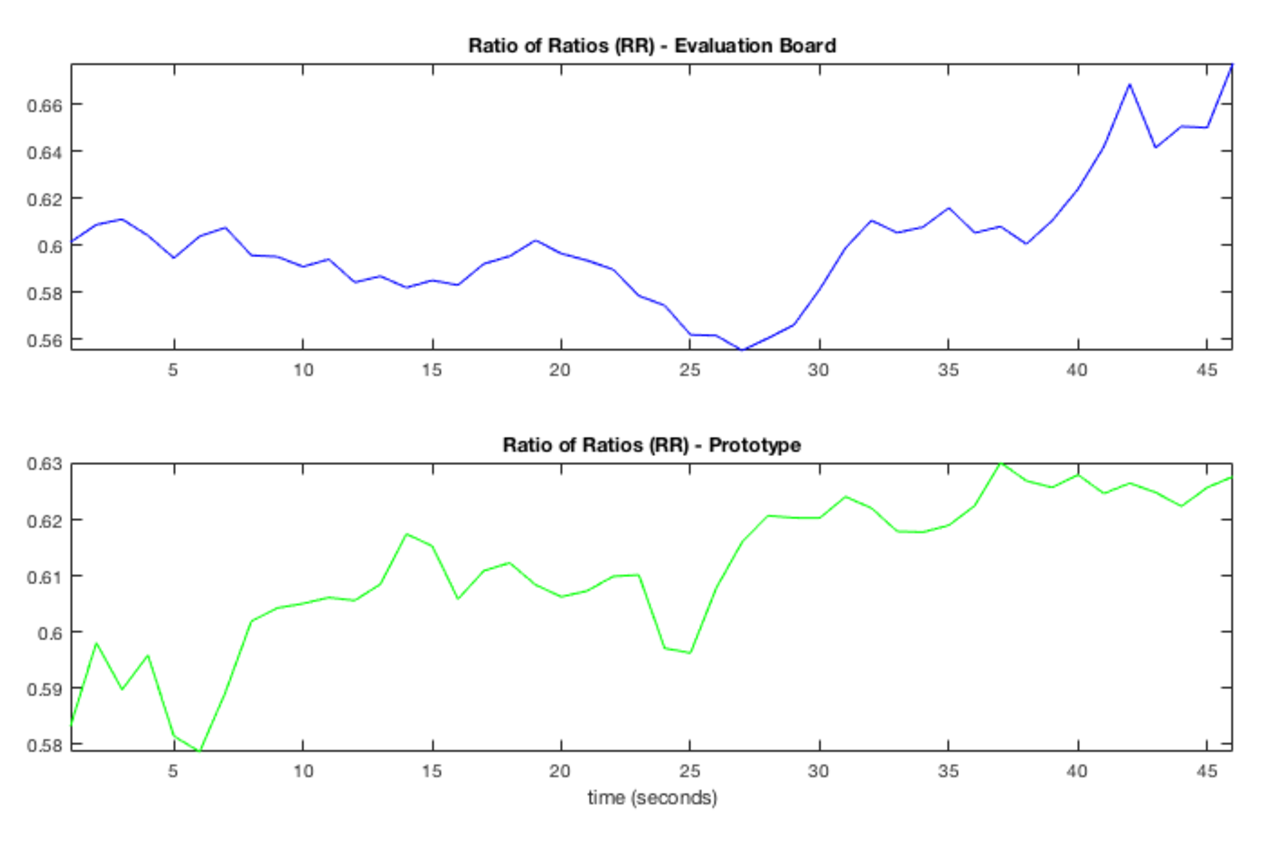
\includegraphics[width=.49\textwidth]{fig/moxi/D1resultsb.pdf}}
    \end{center}
    \caption{(a) EVM and prototype red (red) and infrared (black) PPG signals. (b) Ratio of Ratios in blue (EVM) and green (D1 Device).} 
    \label{fig:D1results}
\end{figure}
To evaluate the D1 prototype, we compared the obtained signals from our device against simultaneously acquired signals from the AFE EVM. The EVM captures PPG signals through transmission via a finger flip on the middle finger. The index finger of the same hand was placed over the optodes on the D1 device. The PPG signals in Figure~\ref{fig:D1resultsa} were simultaneously captured from the D1 device and from the AFE4490 EVM during a 46-second breath holding procedure. Signals were band-pass filtered using a sixth order zero-phase Butterworth filter to remove out of bound noise (0.2 to 5~Hz). As shown in Figure~\ref{fig:D1resultsb}, RR (Equation~\ref{eq:RR}) increases as SpO2 decreases due to the larger difference between extinction coefficients of HbO and HbR at red versus IR light. The pairwise linear correlation coefficient, R, between the two RR signals in Figure 7 is 0.4856. 



%%% Section %%%    
\section{D2: Single Slit Oximeter}
\subsection{D2: Single Slit Hardware}
\begin{figure}
    \begin{center}
    \subfigure[]{\label{fig:D2top}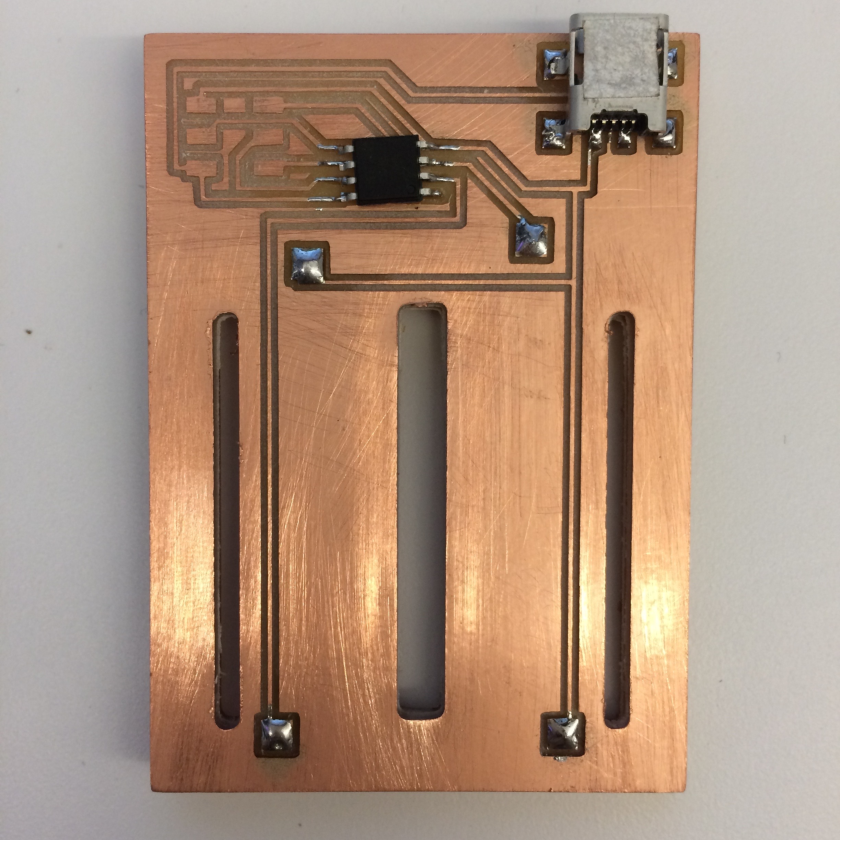
\includegraphics[height=5cm]{fig/moxi/D2top.pdf}}
    \subfigure[]{\label{fig:D2bottom}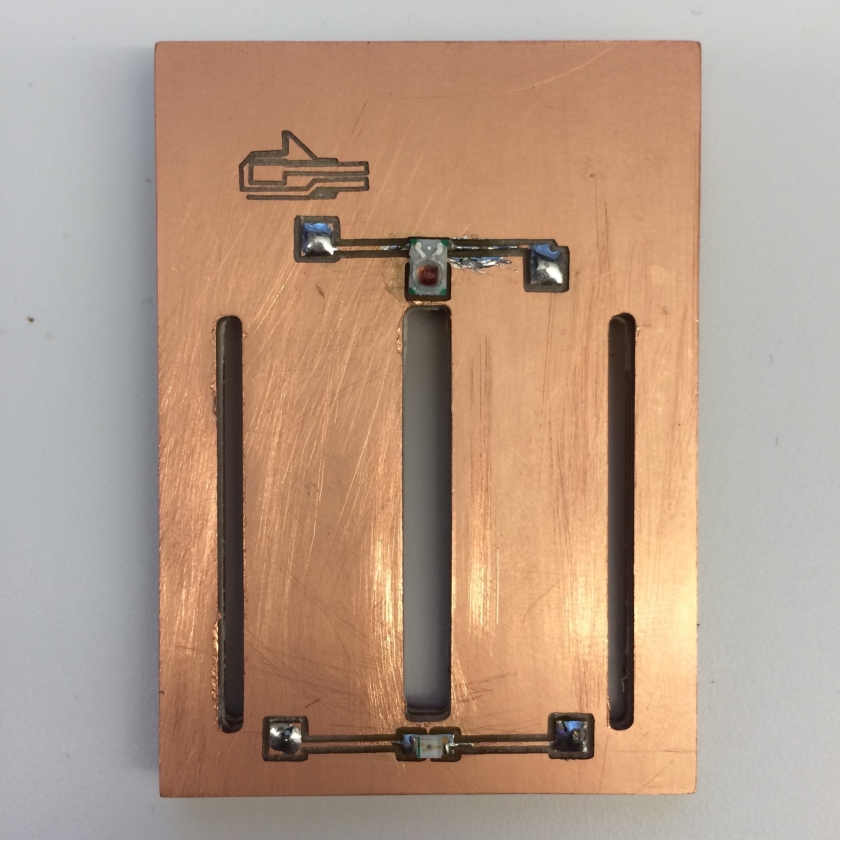
\includegraphics[height=5cm]{fig/moxi/D2bottom.pdf}}
    \subfigure[]{\label{fig:D2on}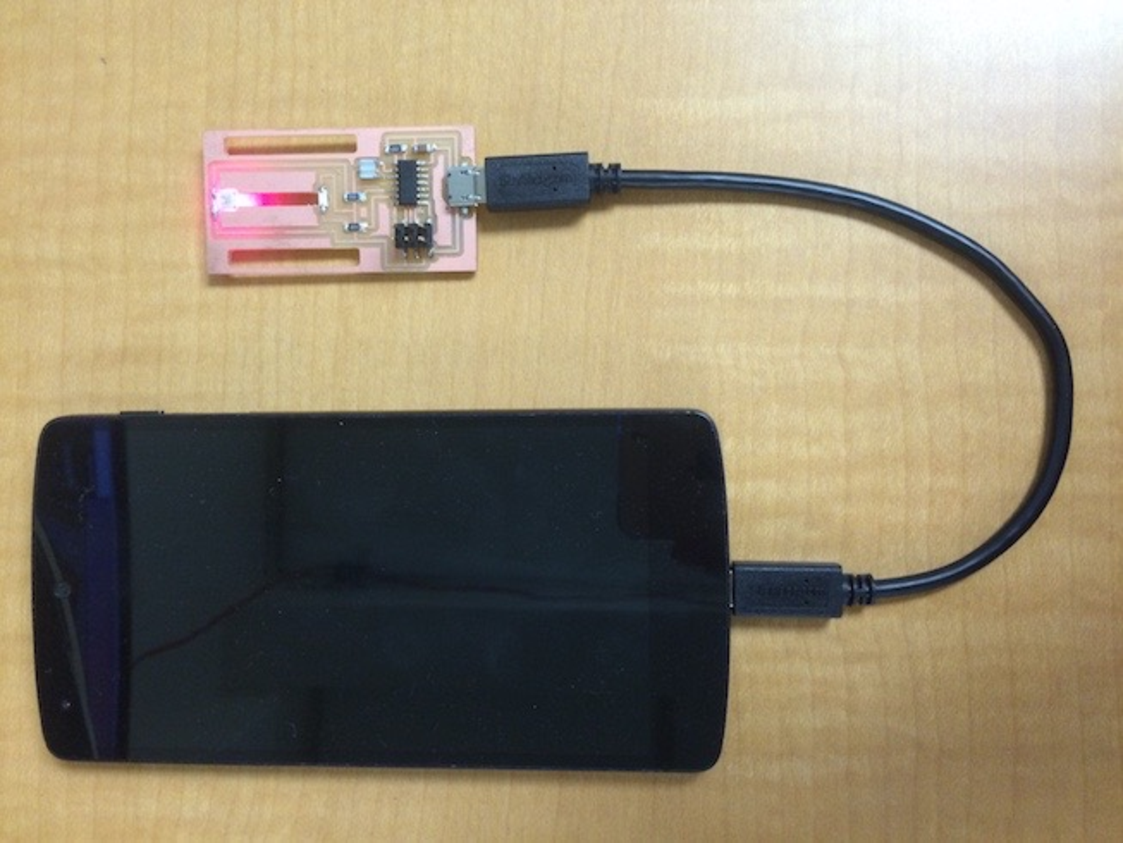
\includegraphics[height=5cm]{fig/moxi/D2on.pdf}}
    \end{center}
    \caption{(a) Top side of D2 circuit showing USB connector and microcontroller. (B) Bottom side of D2 circuit showing deep red (top) and red (bottom LEDs). (C) D2 powered by a smartphone and an on-the-go USB cable.} 
    \label{fig:D2hardware}
\end{figure} 
The D2 design is a compact, low-cost, non-contact, and wearable LED-based illumination module to quantitatively measure tissue oxygenation (StO2). The D2 design is made from a 53x28~mm$^2$ circuit board with a 2x20~mm$^2$ imaging window (the ``slit'') [Figure~\ref{fig:D2top}]. Two LEDs (640 and 730~nm) are mounted facing the skin at opposite sides of the long dimension of the slit [Figure~\ref{fig:D2bottom}]. A 730~nm wavelength was chosen because IR light is not visible in the smartphone CMOS sensor. Moreover, HbO shows a similar absorption at the two wavelengths and HbR has a higher absorption in 640~nm than 730~nm. 

A micro-USB connector is added to provide power while a microcontroller (ATtiny85, Atmel, USA) controls the LED timing [Figure~\ref{fig:D2on}]. Four of the eight pins on the microcontroller are used by the In-Service Programmer (ISP) to program the board using the Master-In-Slave-Out (MISO), Master-Out-Slave-In (MOSI), Serial Clock (SCK), and reset (RST) pins. Power and ground each have a dedicated pin, leaving two analog pins available for the red and deep red LEDs. The use of analog pins allows us to pulse width modulate (PWM) the LEDs. By varying the pulse width, we can control the time an LED is on and control its intensity. The microcontroller has a max output of 40~mA per pin, allowing the LEDs to be connected without the need for resistors. The board is programmed by holding the ISP pins onto the pads without soldering, allowing us to remove the programming pins after programming and reducing the board thickness. In total, the only four components on the D2 milled circuit board are the two LEDs, the microcontroller, and a USB female header for power. 

The D2 design is made of two milled copper boards placed back-to-back. This has two main advantages. First, it allows the ability to easily swap out any broken LEDs if they break during use without having to mill out all the traces. Secondly, the LEDs are soldered directly to the underside of the board, allowing them to be in direct contact with the skin to minimize specular reflection. The entire board is encased inside a 3-D printed PLA cover. Velcro straps on the edges of the milled board allow the D2 design to be comfortable worn [Figure~\ref{fig:D2}]. 

\subsection{D2: Single Slit Software}
The microcontroller is programmed to cycle between three stages at one-second intervals. After securing the module with an elastic Velcro strap and powering the board with a USB cable, the microcontroller automatically begins cycling between the red LED on, deep red LED on, and no LEDs on, each for one second, indefinitely. The one-second interval with no LEDs on is used to capture background data. The diffuse-reflection profile across the slit of both wavelengths can be measured directly by taking a video of the slit opening using the smartphone camera controlled by our Moximeter application. The three intervals from the video stream are automatically detected by comparing intensity values at the ends of the slit. A moving bin average is used to estimate StO2 changes. 

\subsection{D2 Results}
Here, we propose to use the linear slope of the log-scaled image intensity along the slit as a surrogate marker to correlate with tissue oxygenation changes. This slope can be easily computed in real-time on low-power devices such as a mobile phone.
    
\subsubsection{Protocol and Setup}
\begin{figure}
    \begin{center}
    \subfigure[]{\label{fig:D2setup}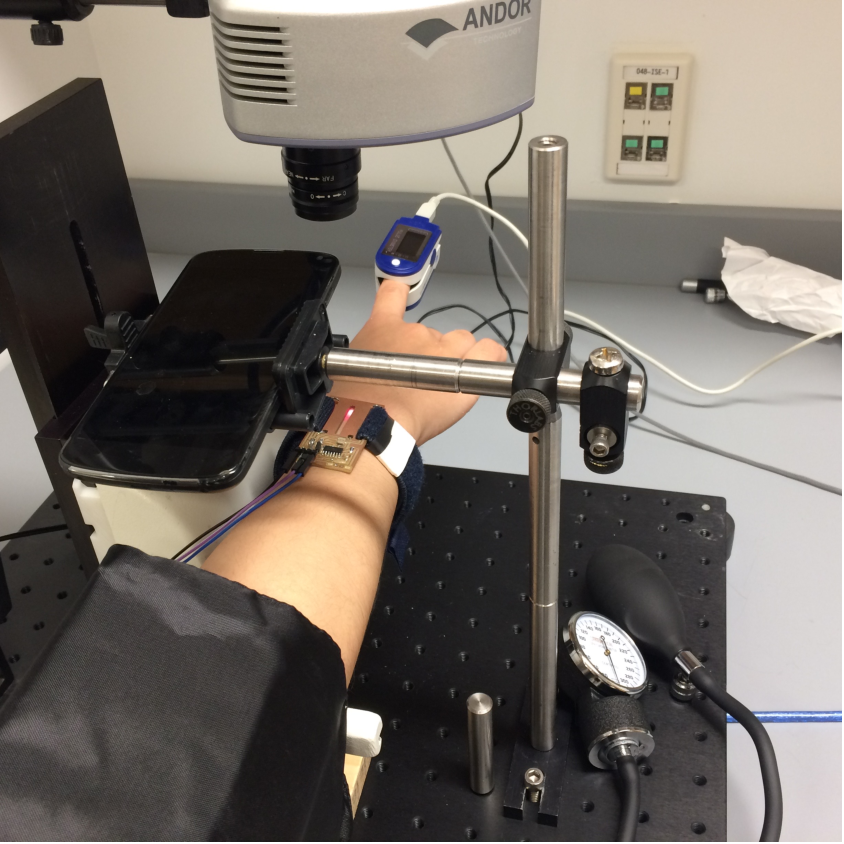
\includegraphics[height=5cm]{fig/moxi/D2setup.pdf}}
    \subfigure[]{\label{fig:D2zoom}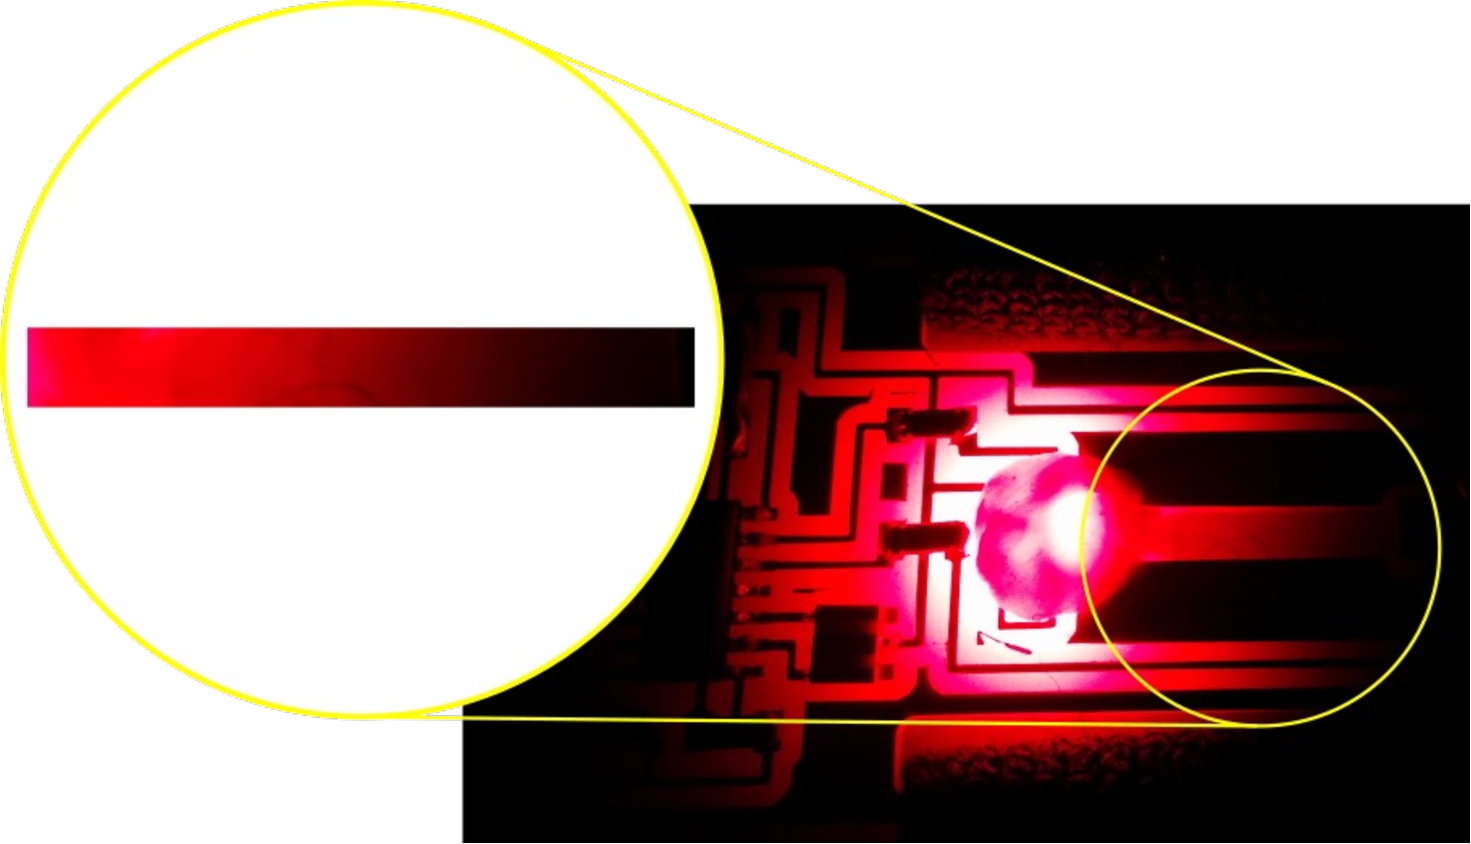
\includegraphics[height=5cm]{fig/moxi/D2zoom.pdf}}
    \end{center}
    \caption{(a) Nexus and Andor camera experimental setup. (b) Example cropped slit image for analysis.} 
    \label{fig:D2protocol}
\end{figure} 
A Nexus 5 Android phone and an Andor Electron Multiplying Charge Coupled Device (EMCCD) camera (Luca-R, Andor, UK) were both mounted above the slit ROI and used to acquire video recordings simultaneously [Figure~\ref{fig:D2setup}]. Cameras recorded at 10.8 (Andor) and 30 (Nexus) frames per second while the red and deep red LEDs alternated every second. Data were captured in a dark room with the phone screen brightness set to the lowest setting. The subject held onto a handle during data gathering to minimize motion artifacts. An example of the acquired image, cropped using MATLAB, can be seen in Figure~\ref{fig:D2zoom}. Slit images were analyzed frame by frame for each camera. A blood occlusion experiment was performed using a standard pressure cuff. Prior to data capture, the pressure was increased to 200~mmHg and held for 20 seconds. After 20 seconds of data capture, the pressure was released. 
        
\subsubsection{Benchtop Results}
\begin{figure}
    \begin{center}
    \subfigure[]{\label{fig:D2resultsa}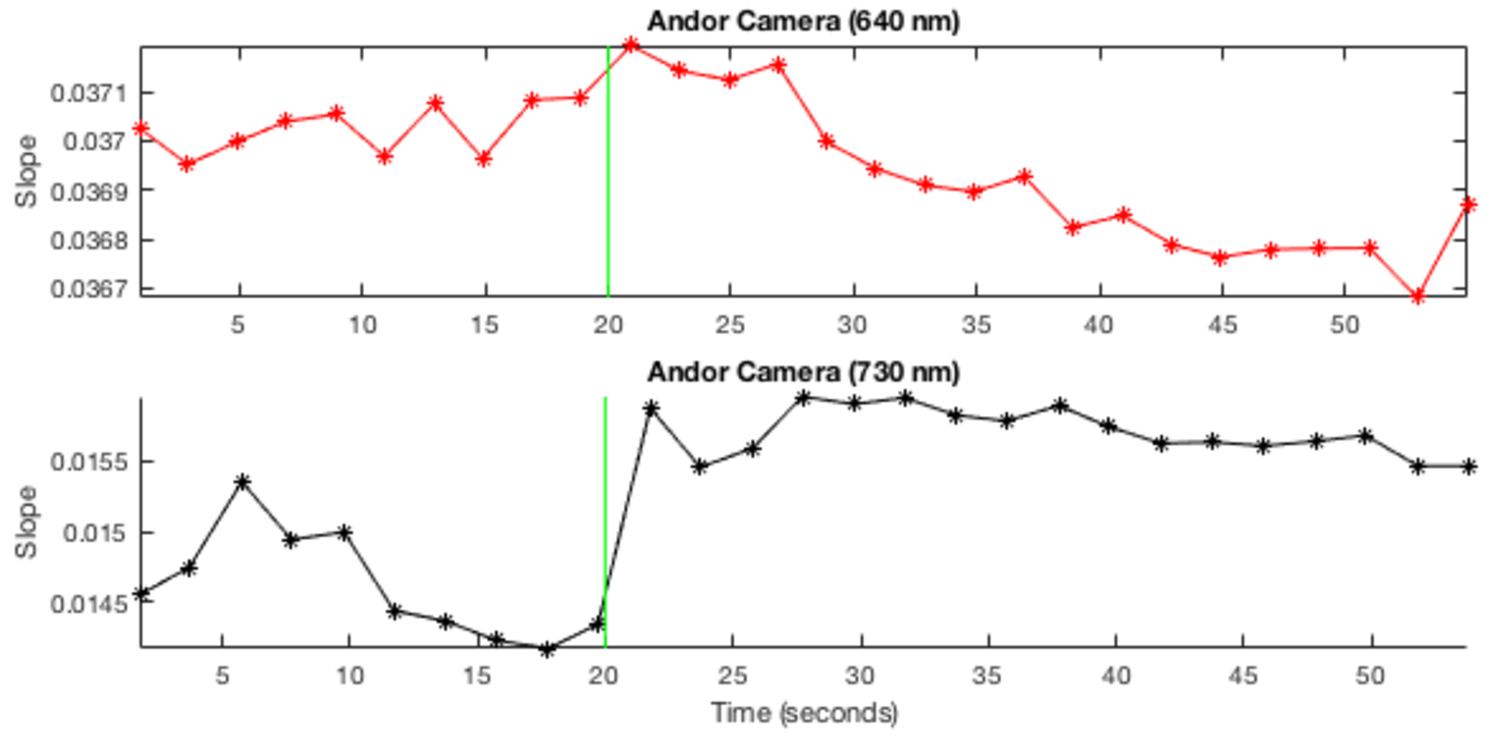
\includegraphics[height=6cm]{fig/moxi/D2resultsa.pdf}}
    \subfigure[]{\label{fig:D2resultsb}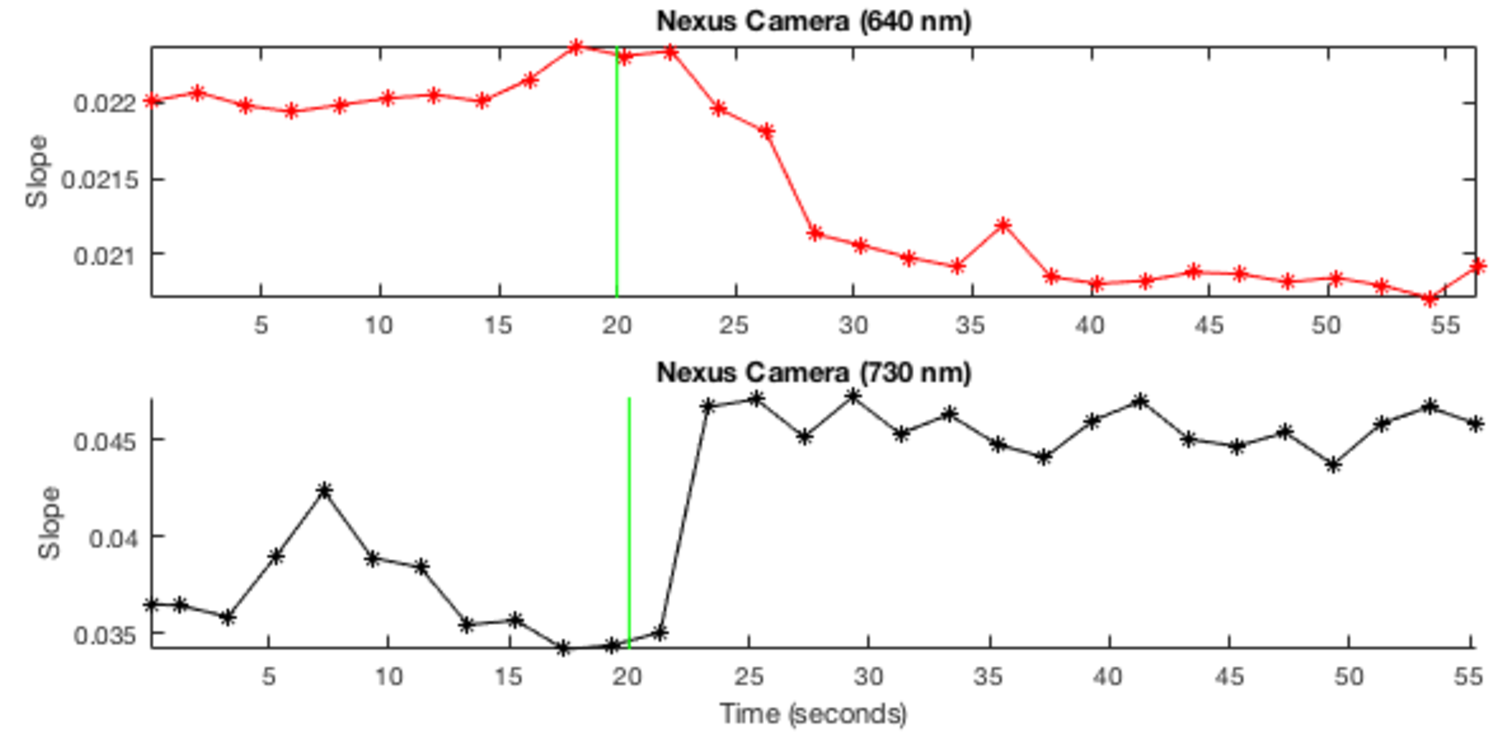
\includegraphics[height=6cm]{fig/moxi/D2resultsb.pdf}}
    \end{center}
    \caption{Intensity attenuation slopes for the Andor (a) and Nexus (b) camera data. Top (640 nm) and bottom (730 nm) rows show the averaged attenuation slope of the log-scaled light intensity over time within a selected window. The vertical green lines mark the point at which pressure from the cuff was released.} 
    \label{fig:D2results}
\end{figure} 
The linear slope time courses obtained from the Andor and Nexus cameras for 640 and 730 nm are shown in Figure~\ref{fig:D2results}. Each marker in the plot is obtained by averaging the frames during the 1 second a particular LED is on. The vertical green line indicates the point of pressure release. The overall shape of the slope profile from the Nexus camera is similar to the Andor camera in both 640 and 730~nm. The pairwise linear correlation coefficients, R, between the two cameras are 0.8627 (640~nm) and 0.7986 (730~nm). The increase in slope immediately following the pressure release is expected due to the higher absorption coefficient of the total hemoglobin that rushes in. These results suggest that a low-cost phone camera is capable of capturing blood volume and oxygenation change in tissue. 



%%% Section %%% 
\section{D3: Paper Filter Pulse Oximeter (MOXI)}
The D3 design is a broadband reflection pulse oximeter that utilizes a smartphone's embedded flash camera LED as the source and the smartphone's camera as a detector. An ultra-low-cost paper filter covering half of the camera's field of view manipulates the original spectra by attenuating certain wavelengths (Figure~\ref{fig:D3inuse}). The hypothesis is that when a finger is placed over the phone's camera and LED, the observed spectra differences combined with the tissue absorption spectra will make it possible to make spectroscopic measurements. Point-of-care devices like these that require no or minimal attachments provide a much greater impact to the accessibility of such devices in resource-poor regions by directly addressing the acquisition and maintenance costs that hinder technological adoption (Table~\ref{tab:lmicbarriers}).

    \subsection{Photon Propagation Simulations}
        \subsubsection{MCXlab simulations}
        \begin{figure}
            \begin{center}
            \subfigure[]{\label{fig:D3inuse}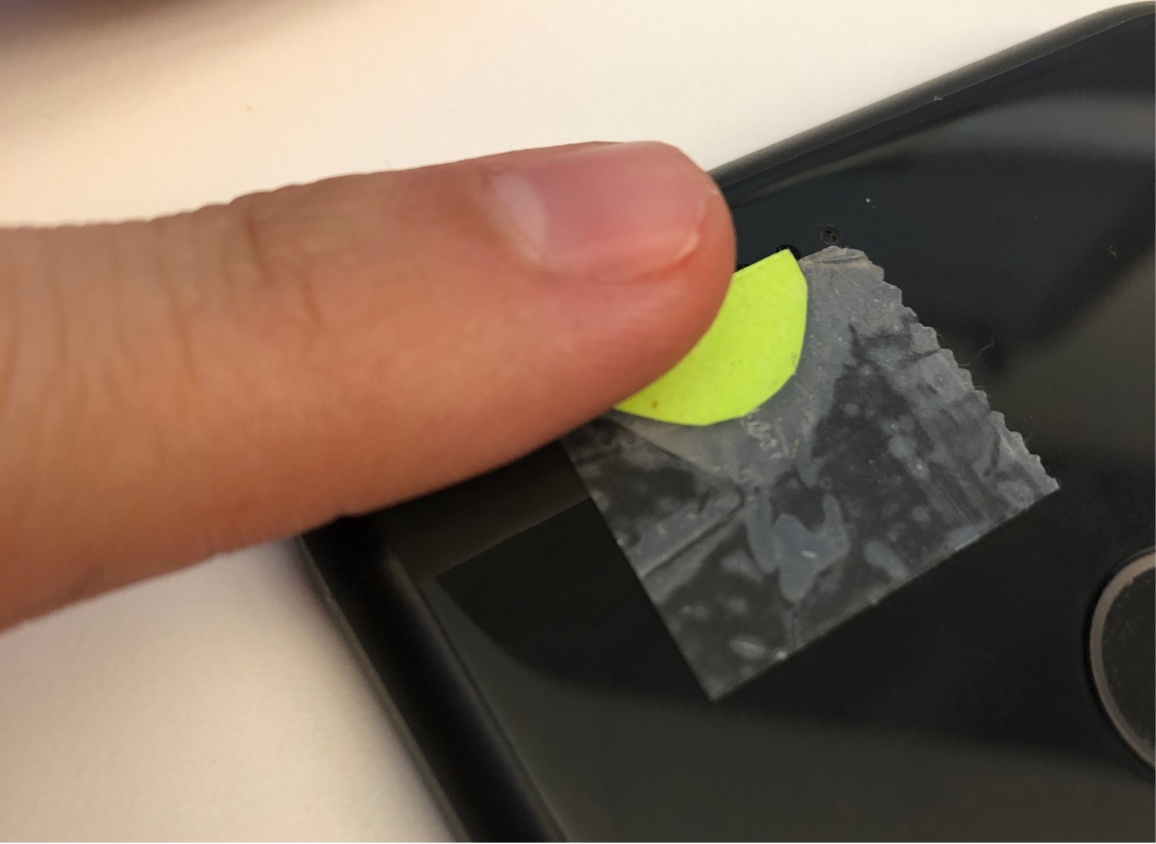
\includegraphics[width=.4\textwidth]{fig/moxi/D3inuse.pdf}}
            \subfigure[]{\label{fig:D3spectra}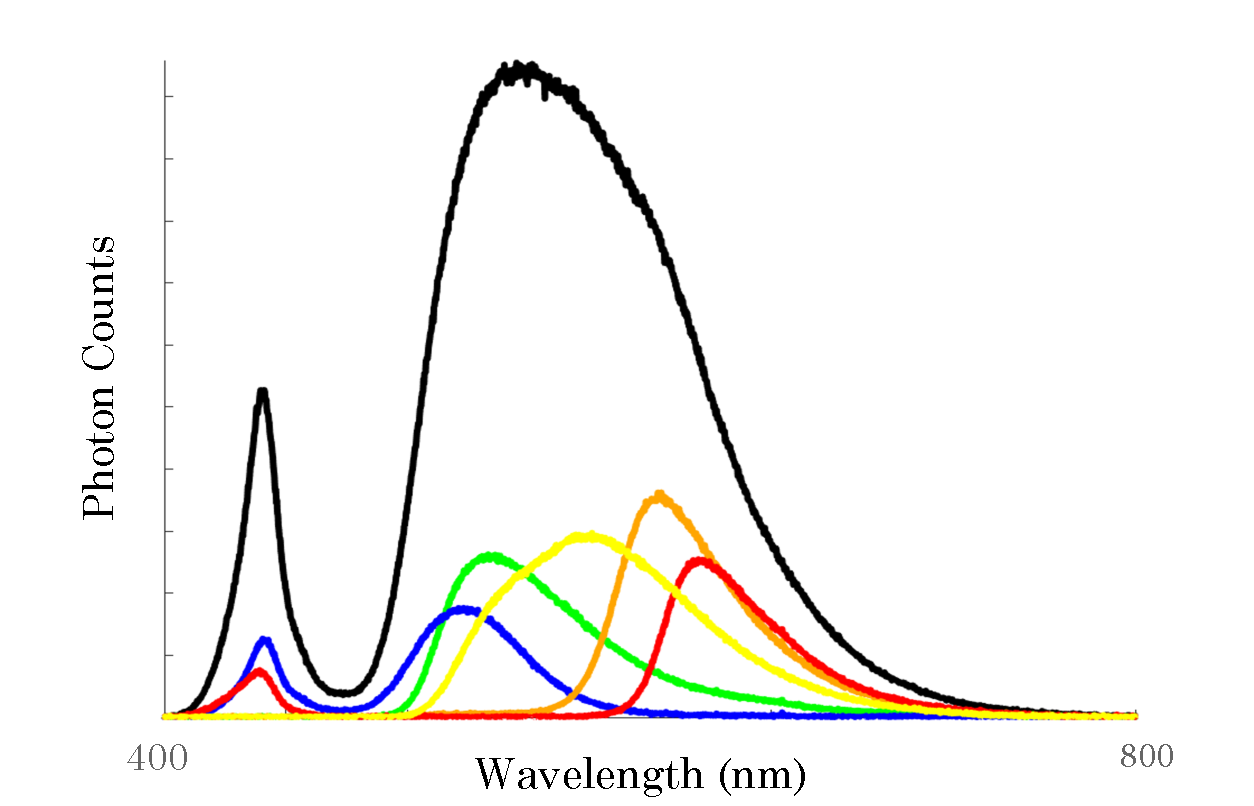
\includegraphics[width=.45\textwidth]{fig/moxi/D3spectra.pdf}}
            \subfigure[]{\label{fig:D3fingersim}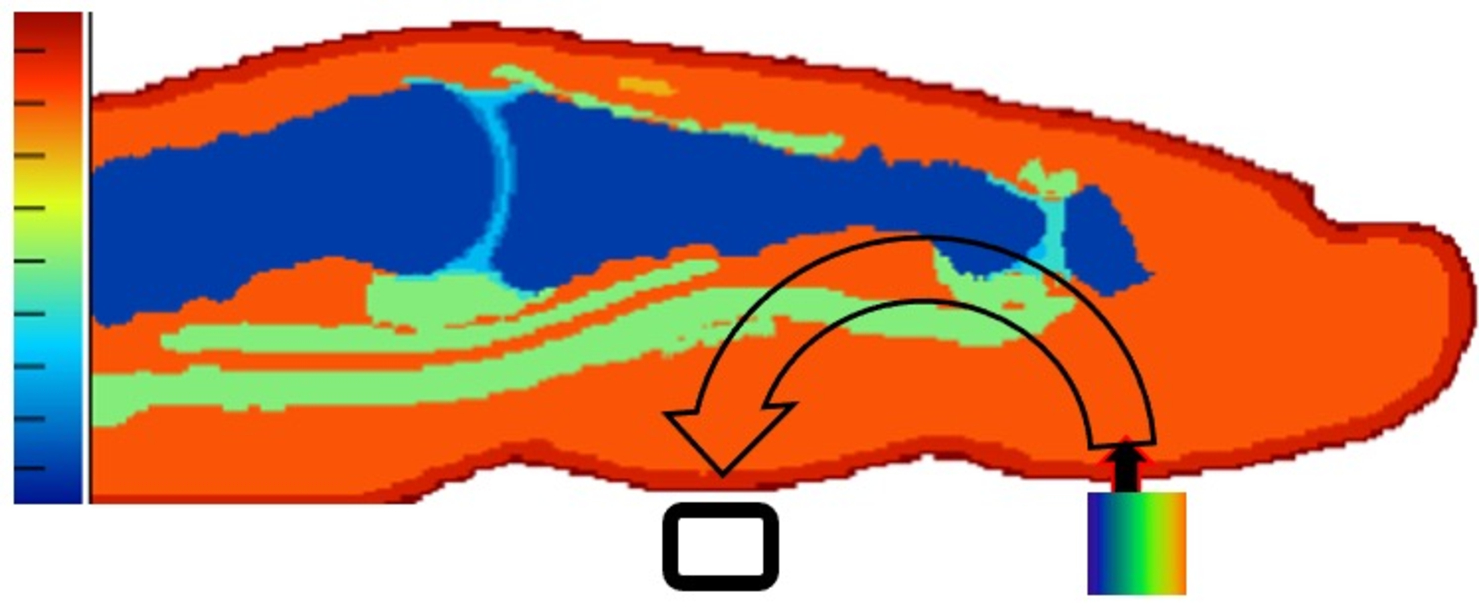
\includegraphics[width=.5\textwidth]{fig/moxi/D3fingersim.pdf}}
            \end{center}
            \caption{(a) D3 design in use with a finger placed over the camera after paper filter is taped over bottom half of mobile phone camera. (b) Broadband spectra (black) and resulting spectra after manipulation using a colored paper filters. The color line refers to the color of the paper filter. (c) Simulation setup showing finger model with six tissue types.} 
            \label{fig:D3simulations}
        \end{figure} 
        A previously segmented, high resolution, 7T realistic 3D finger model was used for the photon propagation simulations~\cite{Laistler2018} [Figure~\ref{fig:D3fingersim}]. Of the original 15 segmented components, the components are combined to represent six tissue types: dermis, epidermis, arteries, veins, fatty tissue, and bone. We ran as series of GPU-based Monte Carlo simulations using Monte Carlo Extreme (MCX)~\cite{Fang2009b} using 5$\times 10^9$ photons in both transmission and reflectance mode. The detector diameter was set to 3~mm, and the source to detector distance in reflectance mode was set to 10~mm, as taken from the mobile phone's dimensions. To simulate broadband light, the optical properties of the finger tissues were swept between the wavelength band of 350 to 1000~nm in 1~nm increments, with intensity based on the measured spectrum of an Android Pixel 2's LED. The filtered broadband light was then further attenuated by the ratio between unfiltered and filtered spectra. Intensity was estimated by fluence.  
        
        \subsubsection{Optical Properties}
        Optical properties of the six tissue types were compiled from literature. The absorption and scattering coefficients of oxygenated whole blood, de-oxygenated whole blood, water, and melanosome were obtained from the MCXYZ.c light transport program~\cite{JacquesMCXYZ}. Bone optical properties were digitized from published results~\cite{KonugoluVenkataSekar2016}. Dermis and epidermis tissue optical properties were created from blood~\cite{Prahl2012}, oxygen~\cite{Jacques2013}, water~\cite{Hale1973}, fat~\cite{VanVeen2004}, and melanosome~\cite{Jacques1991} volume fractions from literature~\cite{Jacques2013}. Blood was assumed to have a hematocrit value of 45\%. The remaining 55\% is plasma, which is typically composed of 92\% water and 8\% food, protein, and other solids~\cite{Jacques2013}, but was simplified to 100\% water for these simulations. Venous blood was assumed to have 70\% SpO2. SpO2 levels ranging from 85\% to 100\% are simulated by adjusting the corresponding optical properties of blood resulting from the volume fractions changes of the arteries. 
        
        \subsubsection{Attenuation Spectra of Paper Filters}
        A spectrometer (Flame VIS-NIR, Ocean Insight, USA) was used to measure the spectrum of an Android Pixel 2 flash LED. Transmission spectra from paper filters of various colors, which further alter the light source spectrum, were also measured [Figure~\ref{fig:D3spectra}]. Broadband spectra was scaled to a max arbitrary unit of 1. The green paper filter was chosen due to its capability of blocking near-infrared light while still not attenuating the original broadband light significantly. This provides a means to differentiate between the broadband light source and a filtered broadband source, which, when combined with the tissue absorption spectra, make spectroscopic measurements using two broadband sources possible. 
        
        \subsubsection{PPG Signal}
        The PPG signal, the measured intensity by the detector, was simulated by increasing the volume of the arteries in the model using a gaussian filter until a 20\% change in the detected fluence was obtained at 690~nm in transmission~\cite{Hertzman1938}. This artery volume increase was used for both transmission and reflection modes as well as for both traditional (two wavelength) and broadband simulations. All other tissue type volumes remained constant. The resulting fluence values for both finger artery volume changes were then used to scale a discretized PPG signal~\cite{Elgendi2012} to create a 60~bpm oscillation optical measurement. A PPG signal was created for each SpO2 value for each pulse oximeter mode (transmission and reflection), as well as for traditional (two wavelength) and broadband simulations (Figure~\ref{fig:D3process}). 
        
        \subsubsection{Ratio-of-ratio for broadband spectroscopy}
        \begin{figure}
            \begin{center}
            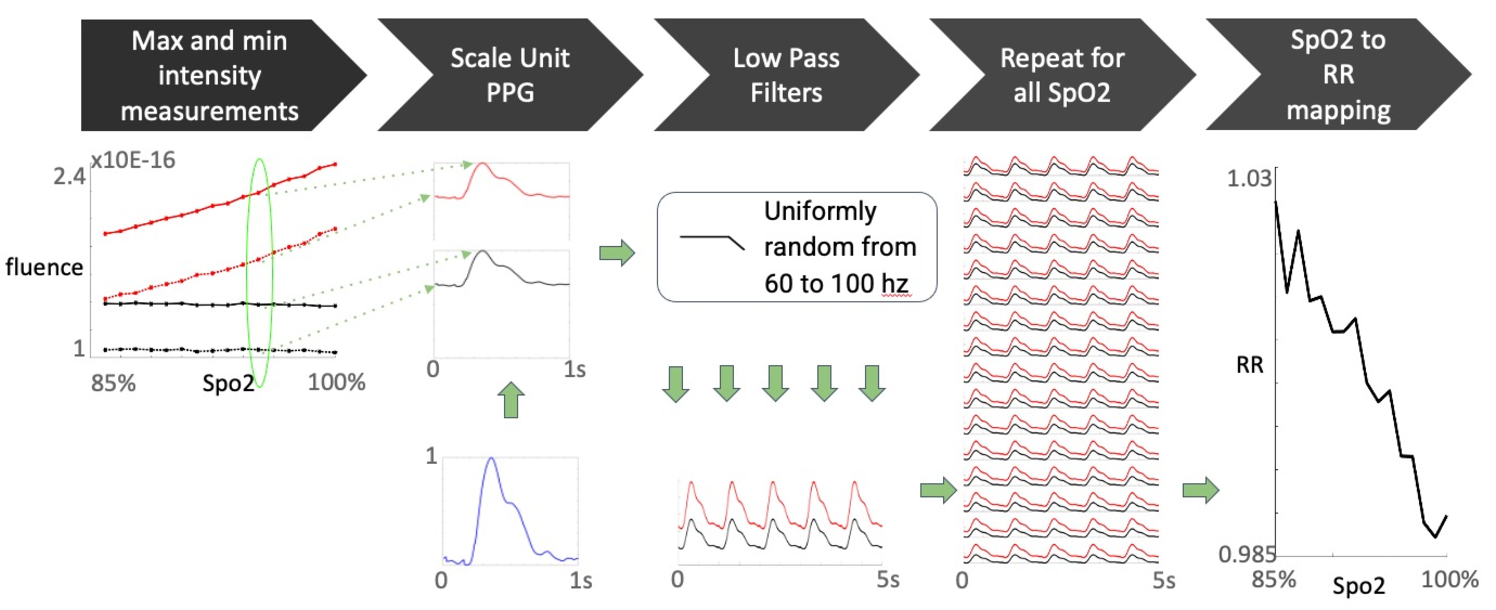
\includegraphics[width=\textwidth]{fig/moxi/D3process.pdf}
            \end{center}
            \caption{Process of creating the ratio-of-ratio to SpO2 mapping in simulation. Monte Carlo simulations result in fluence measurements at various SpO2 values for both wavelengths at 0 and 20\% artery volume increase. An example 1 second PPG pulse is scaled by the fluence measurements and repeated to create a time trace. Each repetition is low-pass filtered with a randomized cutoff frequency between 60 and 100 hz. The RR value is then calculated from the simulated PPG signals.} 
            \label{fig:D3process}
        \end{figure} 
        The traditional calculation of RR was altered slightly to account for broadband light. For this device, RR is defined as 
        \begin{equation} \label{eq:RRbroadband}
            RR = \frac{ A_{BB,AC}/A_{BB,DC} }{ A_{FB,AC}/A_{FB,DC} }
        \end{equation}
        where $A$ the amplitude, BB refers to the broadband PPG signal, and FB refers to the filtered broadband PPG signal of our simulations. 
        
    \subsection{Simulation Validation Results}
    \begin{figure}
        \begin{center}
        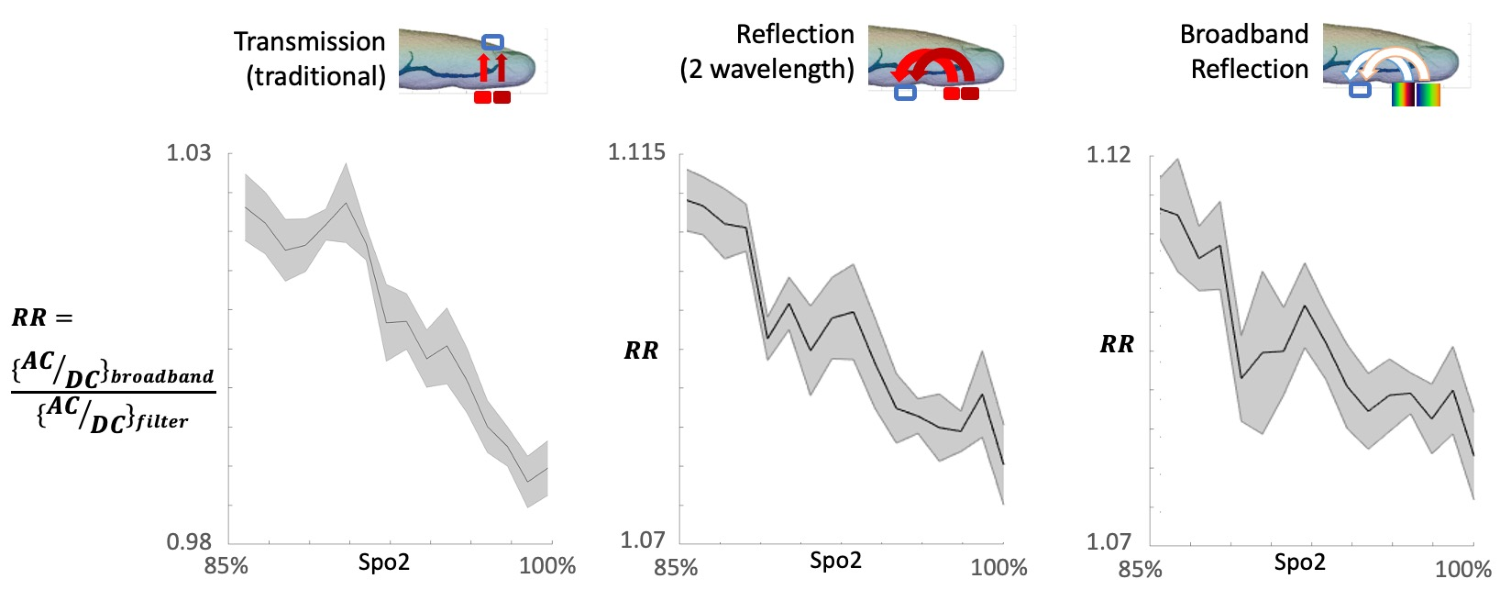
\includegraphics[width=\textwidth]{fig/moxi/D3RR.pdf}
        \end{center}
        \caption{Results of ratio-of-ratio mapping to SpO2 based on Monte Carlo simulations. The curves are shows for two-wavelength simulations in transmission, two-wavelength simulations in reflection, and broadband simulations in reflection.} 
        \label{fig:D3RR}
    \end{figure}
    The RR values calculated from the fluence values at the detector locations from the MCX simulations are shown in Figure~\ref{fig:D3RR}. Traditional two-wavelength transmission simulations showed a typical linearly decreasing relationship between RR and SpO2 as expected. The difference between the maximum and minimum RR is 0.0795. In traditional two-wavelength reflection mode, the range of RR dropped to 0.0519. This indicates that transmission mode is more sensitive to changes in RR, and thus to changes in SpO2, than reflection mode. 
    
    For broadband simulations, the range of RR was 0.013 for transmission mode, dropping by nearly six times as compared to traditional transmission simulations. The difference between RR ranges in traditional and broadband simulations in reflectance mode were about an order of magnitude, with a maximum RR range of 0.005 for broadband reflectance simulations. 
    
    Despite the sensitivity of a traditional two-wavelength transmission pulse oximeter simulation being fifteen times higher than the broadband reflectance simulation, the broadband reflectance simulation relationship between RR and SpO2 is still linear. These results validate our hypothesis that our smartphone-based pulse oximeter can differentiate between SpO2 values using the embedded broadband light from the smartphone's LED, as long as the sensitivity of the smartphone camera is large enough. Additionally, extra care must be taken to block ambient light and reduce motion artifacts to be able to decouple physiological changes from environmental ones. 

    \subsection{Pilot clinical testing}
    A clinical study was designed to simultaneously capture measurements from a mobile phone low-cost paper filter broadband pulse oximeter and a reference device (Rad87, Masimo, USA). The study was conducted on twenty-nine healthy volunteers at the Massachusetts General Hospital Translational Clinical Research Center. 
    
        \subsubsection{Breath-holding procedures}
        The clinical pulse oximeter finger clip was attached to the middle finger of the right arm while the index finger rested on the lens of the Pixel 2 smartphone modified to carry a paper filter that partially covers the lens. Measurements were collected simultaneously using our in-house developed mobile application, Moximeter. Subjects were asked to exhale and then hold their breath for a long as they comfortably could. This was repeated three times, with two minutes to recover in between. Subjects were told to begin breathing immediately if their oxygen saturation according to the clinical pulse oximeter device dropped below 90\%. 
        
        \subsubsection{Data Processing}
        The Moximeter application controlled the smartphone's LED flash and sampled the camera view at 15~Hz. The average pixel intensities of the top and bottom quarter of the camera's image were used to generate the broadband and filtered broadband PPG signals. Moximeter then applies a Chebyshev Type II filter to remove the systemic heart rate signal. The PPG signals are then band-pass filtered using a sixth order zero-phase Butterworth filter to remove out of bound noise (0.2 to 5~Hz). RR is calculated over a 1 second sliding window along the entire time trace. In order to directly compare with the Masimo pulse oximeter, which only outputs SpO2 readings every second, data from the mobile application needed to be converted to SpO2 values. This was done using Dr. Hossein Hakim’s conversion~\cite{Bailey2008}: $SpO2 = 110 - 25\times RR$. This conversion assumes a transmission pulse oximeter. Our clinical dataset was fit to the Masimo pulse oximeter to generate a new SpO2 calibration curve of $SpO2 = 109.59 - 54.69\times RR$. Readings were averaged within 1-second bins to directly compare the 1~Hz Masimo SpO2 values. 
        
        \subsubsection{Pilot Test Results}
        \begin{figure}
            \begin{center}
            \subfigure[]{\label{fig:D3resultsa}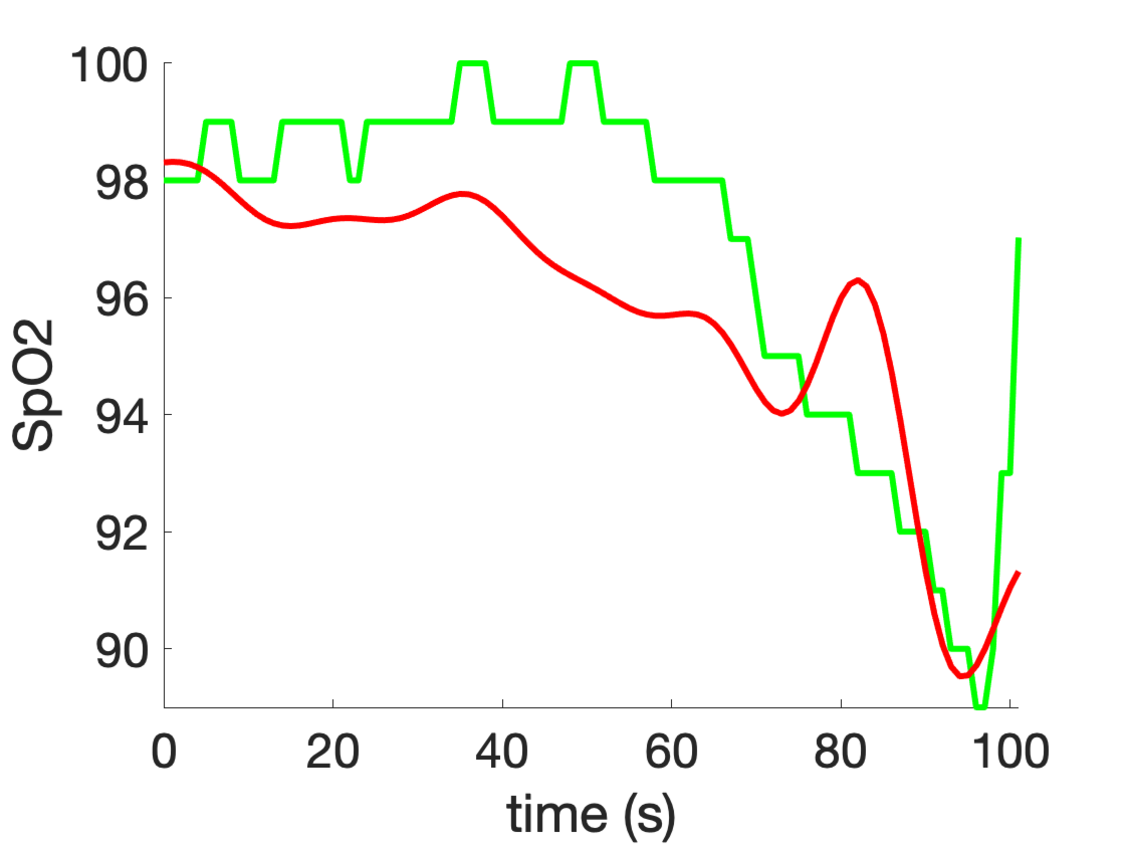
\includegraphics[width=.45\textwidth]{fig/moxi/D3resultsa.pdf}}
            \subfigure[]{\label{fig:D3resultsb}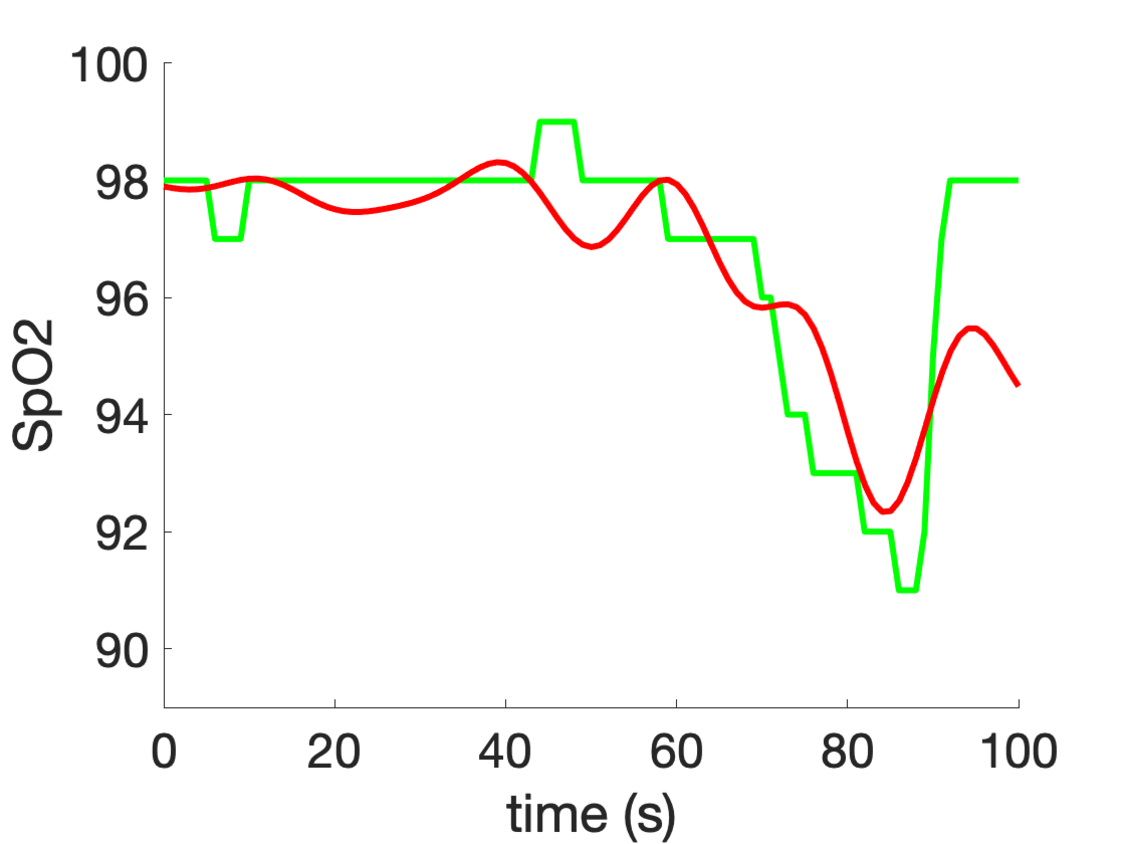
\includegraphics[width=.45\textwidth]{fig/moxi/D3resultsb.pdf}}
            \subfigure[]{\label{fig:D3resultsc}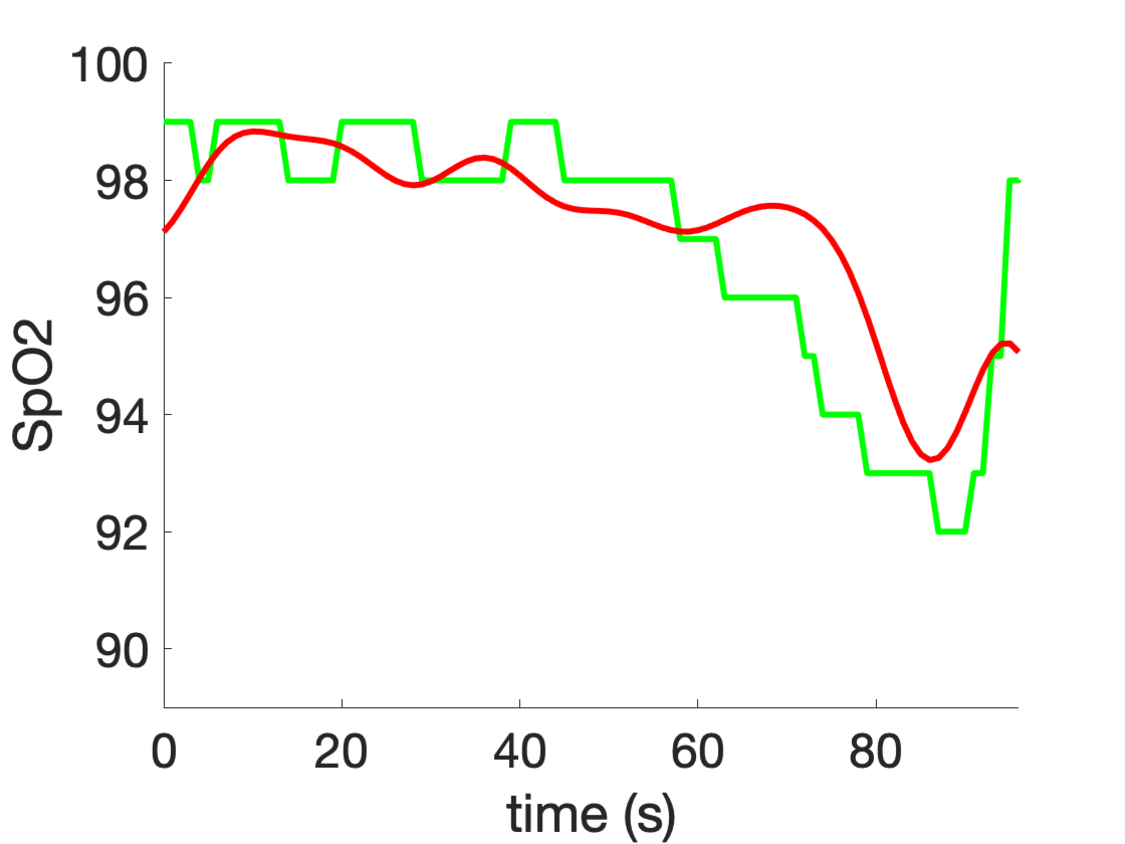
\includegraphics[width=.45\textwidth]{fig/moxi/D3resultsc.pdf}}
            \subfigure[]{\label{fig:D3resultsd}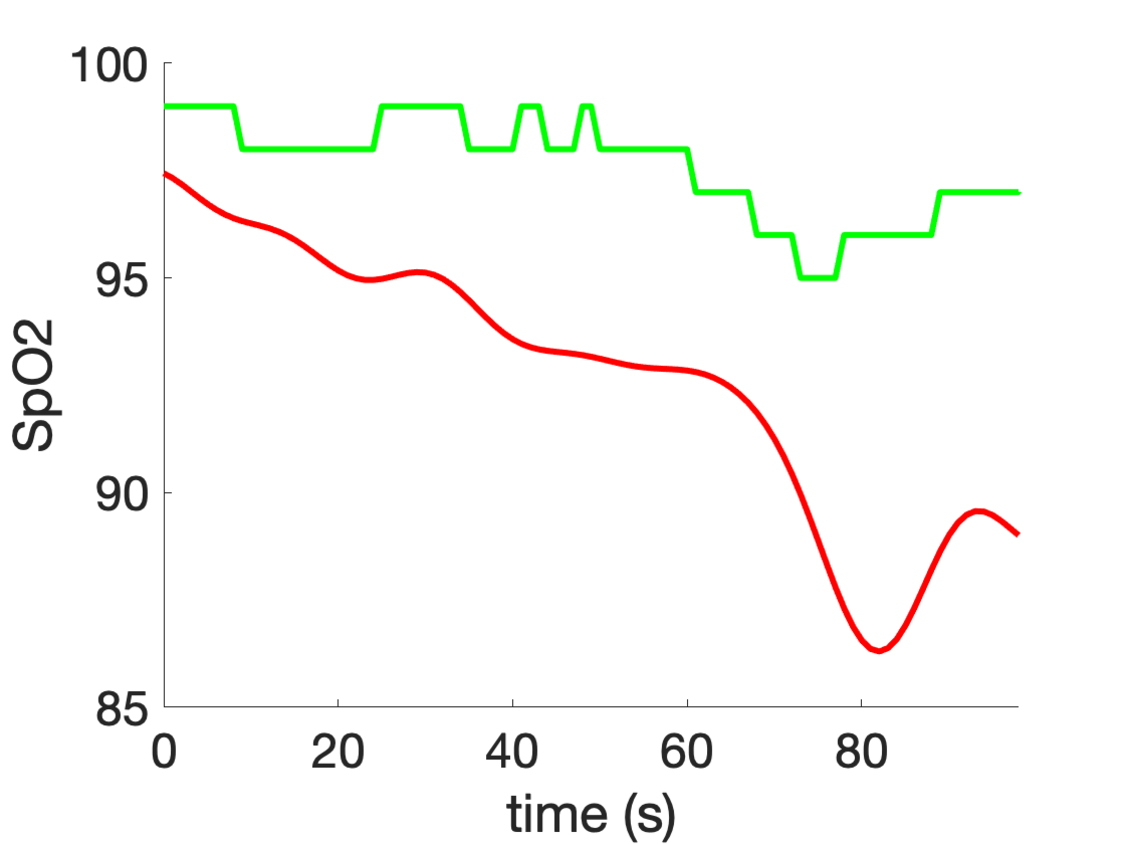
\includegraphics[width=.45\textwidth]{fig/moxi/D3resultsd.pdf}}
            \end{center}
            \caption{Results from comparison of our broadband reflectance-based oximeter with a clinical grade pulse oximeter. Green lines indicate clinical pulse oximeter readings sampled at 1 Hz. Red lines indicate calculated SpO2 measurements using our broadband oximeter. } 
            \label{fig:D3results}
        \end{figure} 
        Selected results from this pilot study are shown in Figure~\ref{fig:D3results}. In many cases [Figures~\ref{fig:D3results}(a), (b), and (c)], we observe a strong overall correlation between SpO2 readings from our paper filter (red lines) and the finger-clip style Masimo clinical grad pulse oximeter readings (green lines). Figure~\ref{fig:D3results} shows that our D3 design captures the expected delay in SpO2 drop after initial breath holding. Additionally, the D3 readings correlate well with the minimum SpO2 values determined by the Masimo baseline. 
        
        In other cases, while the overall trends seem to agree, the range of the SpO2 values differ between the D3 design and the finger-clip oximeter [Figure~\ref{fig:D3resultsd}]. This seems to indicate that the RR to SpO2 conversion may need to be better calibrated. It also indicates that our pulse oximeter prototype may be more susceptible to motion artifacts and noise to alter our SpO2 calculations. 
        
        Due to the low-cost nature of our pulse oximeter, and the inherent motion artifact in broadband based oximeters, the signal variability is quite high. As a result, more advanced signal-processing techniques should be further explored and make these measurements practically useful. Nevertheless, the matching between our ultra-low-cost pulse oximeter readings to the Masimo device in some of the subjects is quite encouraging. 




% --- EOF ---